%
% introduction
\section{Interface}
\label{sec:raspberry-software}
As anticipated, the software run on the Raspberry Pi is made following the
paradigm of object-oriented programming. Made in C++/Qt making extensive use
of the proprietary classes of the framework and the Standard Template Library
(STL). This program has some dependencies with regard to the thermal camera
drivers supplied by the manufacturer and are 32-bit, since the Raspberry Pi 3,
described in \ref{sec:raspi3}, is equipped with a 32-bit ARM Cortex-A53
processor. These allow total control of the camera. The second dependency is the
Raspicam library which allows the interface with the RGB camera allowing the
image acquisition.
%
\begin{figure}[htb]
	\centering
	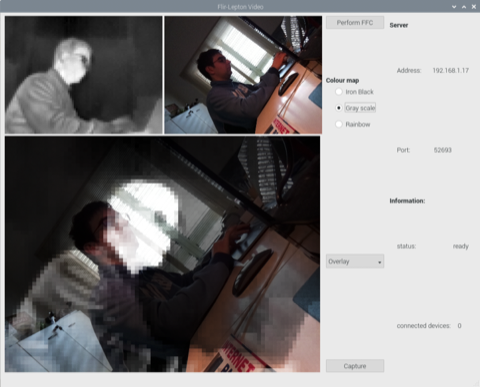
\includegraphics[width=0.65\textwidth]{grayscale.png}
	\caption{User interface run on Raspberry Pi 3b.}
	\label{fig:software-main-ui}
\end{figure}
%
% interface
Continuing a user interface has been created through the use of widgets, this is
divided into three areas. The first area shows the video streams acquired
separately in two labels, the third larger label shows the two streams mixed
through filters made available as default the overlay filter is used. It was
preferred not to perform a match of the images with pixel-by-pixel recalculation
for two reasons: the first due to the high difference in size of the sensors as
that of the thermal camera is $80 \times 60$ pixels while the Raspicam is $3280
\times 2464$ pixels. The second is to not aggravate the computational load on
the CPU.\\\linebreak
The second area provides some controls for the user, in fact it is
possible to save thermal images on files during the acquisition. you can change
the heat map applied to the image on the fly by choosing from three different
possibilities, in the figure you can observe the result. 
Finally, it is possible to modify the mixing filter, also on the fly, of the
video streams to obtain different effects to improve visibility or to increase
details.\\
The last section of the user interface shows the information relating
to the TCP socket used for sending the video stream to other devices.
%
% image ui
\begin{figure}[htb]
    \centering
    \subfloat[][\emph{lava}.\label{subfig:lava-map}]
        {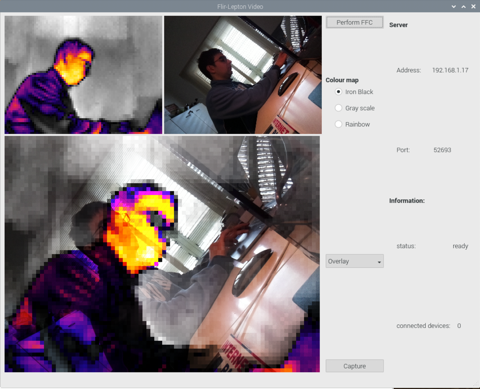
\includegraphics[width=.30\textwidth]{lava.png}} \quad
    \subfloat[][\emph{grayscale}.\label{subfig:grayscale-map}]
        {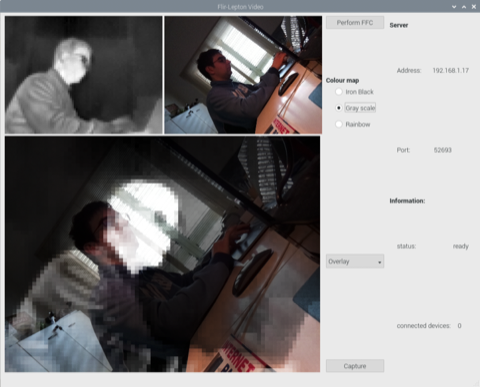
\includegraphics[width=.30\textwidth]{grayscale.png}} \quad
    \subfloat[][\emph{rainbow}.\label{subfig:rainbow-map}]
        {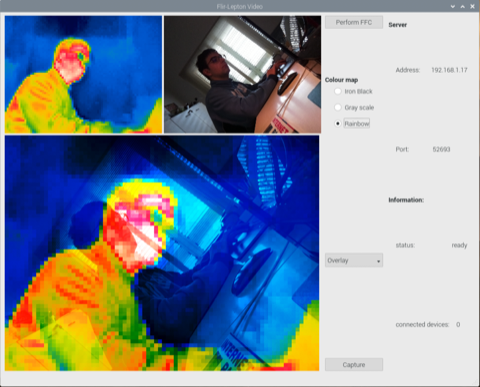
\includegraphics[width=.30\textwidth]{rainbow.png}}
    \caption{Result colourization applied to thermal camera data.}
    \label{fig:reuslt-maps}
\end{figure}
%
% software analysis 
\subsection{Software Analysis}
\label{ssec:raspberry-softw-analysis}
The user interface is run on the main thread, in order to maximize the
performance of the executed code the image acquisition operation is performed in
the secondary thread. Thanks to the use of the signal and slot system of Qt it
is possible to update the labels without blocks typical of multi-threaded
programming. 
The difficulty of concurrent programming usually consists in
synchronizing the access to resources by different threads that act in
competition on the same resources. Having two or more threads accessing the same
data simultaneously can lead to unexpected and unwanted results. 
In fact, without the application of particular programming techniques, it is not
possible to predict in a deterministic way, at the time of execution, when that
specific thread will be executed: their progression depends on the priorities
decided by the scheduler of the operating system and not by the programmer. 
In fact, multiple threads can access the same variable and modify its content or
value. Therefore, synchronization techniques such as mutual exclusion are used
to solve the problem. As a result, ideally a thread should execute code as
independent of the rest of the program as possible. Furthermore, errors in
synchronization between threads are often very difficult to detect because their
occurrence essentially depends on the environment in which the program is run.
The synchronization of one thread with another is normally necessary to allow
them to communicate with each other and to return the results of a function to
the main process; it is normally done through \emph{mutex}\cite{wiki:thread}.
Analysing the code of the thread that takes care of acquiring the images we can 
see that it proceeds without mutex\footnote{The mutex class is a synchronization
primitive that can be used to protect shared data from being simultaneously
accessed by multiple threads.}, but uses the signal and slot system as mentioned
before.
%
% code list
\begin{listing}[ht]
\inputminted[bgcolor=bg,frame=lines,framesep=2mm, linenos=true, autogobble, breaklines=true, fontsize=\scriptsize, firstline=36, lastline=100]{c++}{software/code/leptonthread.cpp} 
\caption{Infinite loop thread cameras.}
\label{lst:rasp-leptonthread}
\end{listing}
%
Going to analyse in detail the infinite loop, reported in the
listing (\ref{lst:rasp-leptonthread}), executed in a thread other than the main
one that manages only the main interface, it can be observed that:
\begin{itemize}
\item When the function starts, an instance of the QImage type object is
instantiated to contain the image acquired during the cycle. The parameters of the
frame size are provided and the color space this allows to increase the speed of
the cycle as it will not be cyclically cancelled and reallocated the same, but
will be reused. The communication with the thermal camera is opened via the SPI
port if the cycle is not started or if the communication is interrupted the
communication is closed.
% code list
%\begin{minipage}{\linewidth}
%\centering
%\inputminted[bgcolor=bg,frame=lines,framesep=2mm, linenos=true, autogobble, breaklines=true, fontsize=\scriptsize, firstline=36, lastline=61]{c++}{software/code/leptonthread.cpp} 
%\captionof{listing}{Data acquisition from SPI.}
%\label{lst:rasp-leptonthread-data} 
%\end{minipage}
%
\item The main cycle is to acquire data from the saved camera registers, as the
order is MSB\footnote{MSB can also stand for "most significant byte".
\emph{Big-endian processor}: When data is loaded into a multi-byte register, the
first byte (with the lowest address) is the most significant byte of the
data.\cite{56322}}, reversed in according to LSB\footnote{LSB can also stand
for "least significant byte". \emph{Little-endian processor}: When data is
loaded into a multi-byte register, the first byte (with the lowest address) is
the least significant byte of the data.\cite{56322}}. The values are then scaled
to obtain a consistent representation of the hot and cold areas. Then the color
map is applied to color the raw data obtained from the scaling process described
above.
%% code list
%\begin{minipage}{\linewidth}
%\centering 
%\inputminted[bgcolor=bg,frame=lines,framesep=2mm, linenos=true, autogobble, breaklines=true, fontsize=\scriptsize, firstline=79, lastline=108]{c++}{software/code/leptonthread.cpp} 
%\captionof{listing}{Flip the MSB and LSB and colouration.} 
%\label{lst:rasp-leptonthread-MSB-LSB} 
%\end{minipage}\linebreak
%%
\item Finally, signals are output for the coloured thermal image, for the RGB
image acquired by the Raspicam library and passed through the slot and the last
resulting from mixing of previous two depend on effect of selected in UI interface.
%% code list
%\begin{minipage}{\linewidth}
%\centering 
%\inputminted[bgcolor=bg,frame=lines,framesep=2mm, linenos=true, autogobble, breaklines=true, fontsize=\scriptsize, firstline=36, lastline=117]{c++}{software/code/leptonthread.cpp} 
%\captionof{listing}{Infinite loop thread cameras.} 
%\label{lst:rasp-leptonthread} 
%\end{minipage}
\end{itemize}
As can be seen, the cycle proceeds without mutuals or blocking conditions, in
fact, as previously described, it is possible to change the color map or the
mixing tool on the fly.
%
% analysing comunication
% description socket tcp
\subsection{TCP communication}
\label{ssec:software-TCPSocket}

% code list
\begin{listing}
\inputminted[bgcolor=bg,frame=lines,framesep=2mm, linenos=true, autogobble, breaklines=true, fontsize=\scriptsize, firstline=84, lastline=95]{c++}{software/code/mainwindow.cpp} 
\caption{Particular report function sending image.} 
\label{lst:rasp-code-thread} 
\end{listing}
%
% % code list
% \begin{listing}[ht] 
% \inputminted[bgcolor=bg,frame=lines,framesep=2mm, linenos=true, autogobble, breaklines=true, fontsize=\scriptsize]{c++}{software/code/streamthread.cpp} 
% \caption{Infinite loop stream thread.} 
% \label{lst:streamthread} 
% \end{listing}
%

